\chapter{Spatially-Dependent Material Uncertainties in Anisotropic Nonlinear Elasticity: Stochastic Modeling, Identification, and Propagation}
\label{chap:artery}

An underlying Gaussian measure, usually reduced by means of a Karhunen-Lo\`{e}ve expansion (to tackle the so-called curse of dimensionality) and pushed-forward by a given (e.g., exponential) transformation (to ensure almost sure positiveness as coefficient in an elliptic operator for instance), is usually invoked for heterogeneous inputs, described as random fields \cite{Ghanem1991,Ghanem2017}. Alternatively, input probability measures for constitutive models may be \textit{implicitly} described through scale-bridging procedures where microstructural features are modeled \cite{Sobczyk,Torquato}, homogenized at mesoscale \cite{OstojaBook, ostoja1998, baxter2001a, baxter2001b, STEFANOU2017319}, and potentially integrated within generic frameworks for dimensionality reduction \cite{BESSA2017633} and materials design \cite{Yin2009}. Such approaches can provide more realistic descriptions of material variability, owing to the fact that they rely on a mechanistic, multiscale-informed generator for the stochastic inputs.

Modeling contributions in the context of nonlinear behavior are far more scarce. As with the case of linear elasticity, implicit descriptions can be obtained through computational homogenization; see \cite{Clement2012,Clement2013} for hyperelastic microstructures, and \cite{OZTURK2021104294} for plasticity. Another approach aimed at prescribing dependencies evaluated through the statistical treatment of a digital database on hyperelastic solids was reported in \cite{caylak2018stochastic}. The first attempts to construct stochastic models for hyperelastic materials based on information theory can be found in \cite{staber2015stochastic} and \cite{Staber2017zamm} for the incompressible and compressible (homogeneous) cases, respectively. Here, constraints related to polyconvexity and linearization at small strains were considered to ensure well-posedness and introduce statistical dependencies between the primary material parameters. Such models were used to identify the probabilistic behavior of soft biological tissues based on physical experiments in \cite{STABER2017743}, and to investigate a series of theoretical propagation problems in \cite{Mihai-1, Mihai-2, Mihai-3, Mihai-4} (see also \cite{mihai2018stochastic}). These developments served as the basis to address the heterogeneous case, where properties are allowed to vary spatially, in \cite{STABER201894}. In addition to admissibility, the model also enforced the structural compliance of the covariance kernel on patient-specific geometries by relying on noise filtering---a technique that we will use in this paper as well. The methodology was later used in \cite{staber2019stochastic} to identify fluctuations in the anisotropic strain energy density function defining a composite laminate. Finally, a Bayesian approach relying on a regular covariance kernel (evaluated with the Euclidean metric) was proposed in \cite{Biehler2015}; see also \cite{fitt2019uncertainty} for Bayesian model selection for the homogeneous case. 

We restrict the analysis to the passive mechanical response of the artery: the integration of the active component, which can play an important role in vivo \cite{YOSIBASH201251}, is left for future study. To the authors' best knowledge, this represents the first contribution where both the stochastic model and the calibrated hyperparameters are presented in a self-contained manner. This may, in particular, support the development of data-driven frameworks, which are increasingly used to model and classify the behavior of such soft biological tissues (see \cite{Holzapfel2021} as an example). It is also important to note that the methodology of construction is applicable for modeling other classes of materials, such as engineered composite laminates that can be experimentally characterized through full-field measurement techniques.

This section is structured as follows. In Section~\ref{sec:background-det-nonlin}, we recall the necessary background pertaining to constitutive modeling in finite elasticity. In Section~\ref{sec:sto-homogeneous}, we address the modeling of stochastic stored energy functions parameterized by homogeneous random coefficients. These results are subsequently invoked and extended in Section \ref{sec:sto-heterogeneous} where we consider the case of spatially-dependent material parameters, modeled as non-Gaussian random fields. Calibration aspects are discussed in Section \ref{sec:calibration}, using physical experiments taken from the literature. Uncertainty propagation on patient-specific geometries is finally conducted in Section \ref{sec:uncertainty-propagation}.

\section{Background in Nonlinear Elasticity}
\label{sec:background-det-nonlin}


\subsection{Elasticity Tensor at Small Strains} \label{Linearization}
We conclude this section by deriving the linearized elasticity tensor at small strains associated with the deterministic strain energy density function $\psi$. This calculation will be used, in Section \ref{sec:sto-homogeneous}, to introduce suitable constraints, as well as an ad hoc parameterization, in the stochastic models. The small strain elasticity tensor is denoted by $\mathbb{C}$ and is defined as (see \cite{Holzapfel-Book-2000} for instance)
\begin{equation}
    \mathbb{C} = \left.4\frac{\partial^2 \psi}{\partial \bfC \partial \bfC}\right\vert_{\bfC = \bfI}\,. \label{eq:elasticity-def}
\end{equation}
Following Eq.~\ref{eq: strain energy density function}, we introduce the decomposition
\begin{equation}
    \mathbb{C} = \mathbb{C}^{MR} + \mathbb{C}^{p} + \mathbb{C}^{ti}
\end{equation}
with
\begin{equation}
    \mathbb{C}^{\text{MR}} = \left.4\frac{\partial^2 \psi^{\text{MR}}}{\partial \bfC \partial \bfC}\right\vert_{\bfC = \bfI}\,, \quad
    \mathbb{C}^{\text{p}} = \left.4\frac{\partial^2 \psi^{\text{p}}}{\partial \bfC \partial \bfC}\right\vert_{\bfC = \bfI}\,, \quad
    \mathbb{C}^{\text{ti}} = \left.4\frac{\partial^2(\psi_{(1)}^{\text{ti}} + \psi_{(2)}^{\text{ti}})}{\partial \bfC \partial \bfC}\right\vert_{\bfC = \bfI}\,.
\end{equation}
Proceeding with standard tensor calculus, we obtain
\begin{equation}
    \mathbb{C}^{\text{MR}} = (4 \mu_1 + 6 \sqrt{3} \mu_2) \mathbb{K}\,, \quad \mathbb{C}^{\text{p}} = 6 \mu_3 \beta_3^2 \mathbb{J}\,, \quad \mathbb{C}^{\text{ti}} = 48 \mu_4(1-\rho)\mathbb{J}\,,
\end{equation}
where $\mathbb{J}$ and $\mathbb{K}$ are the standard basis tensors for the set of isotropic tensors, given by
\begin{equation}
    \mathbb{J}_{ijk\ell} = (1/3) \delta_{ij} \delta_{k\ell}\,, \quad \mathbb{K}_{ijk\ell} = \mathbb{I}_{ijk\ell} - \mathbb{J}_{ijk\ell}\,,
\end{equation}
with $\mathbb{I}$ the fourth-order symmetric identity tensor, defined as $\mathbb{I}_{ijk\ell} = (\delta_{ik}\delta_{j\ell}+\delta_{i\ell}\delta_{jk})/2$. The total contribution therefore writes as
\begin{equation}
    \mathbb{C} = (6 \mu_3 \beta_3^2+48 \mu_4(1 - \rho))\mathbb{J} + (4\mu_1+6\sqrt{3}\mu_2) \mathbb{K}\,. \label{eq:elasticity}
\end{equation}
Eq.~\eqref{eq:elasticity} indicates that the model exhibits isotropy at small strains and can thus be rewritten as
\begin{equation}
    \mathbb{C} = 3 c_1 \mathbb{J} + 2 c_2\mathbb{K}\,,
\end{equation}
where $c_1$ and $c_2$ are identified as the bulk and shear moduli, respectively:
\begin{equation}
    c_1 = 2 \mu_3 \beta_3^2+16\mu_4(1-\rho)\,,\quad c_2 = 2\mu_1+3\sqrt{3}\mu_2\,.
\end{equation}
The above relationships can be used to express $\mu_2$ and $\mu_4$ in terms of the remaining variables, yielding
\begin{equation}
     \mu_2 = 3^{-3/2}(c_2 - 2\mu_1)\,, \quad \mu_4 = (c_1 - 2 \mu_3 \beta_3^2)/\left(16(1-\rho)\right)\,.
\end{equation}
For later use, it is convenient to introduce two auxiliary variables $u$ and $v$ defined as
\begin{equation}
    u = 2\mu_1/c_2\,, \quad v = c_1 - 2 \mu_3 \beta_3^2\,,
\end{equation}
so that 
\begin{equation}
    \mu_2 = 3^{-3/2} c_2 (1 - u)\,, \quad \mu_4 = v/\left(16(1-\rho)\right)\,.
\end{equation}
It should be observed that by construction, $u \in \, ]0,1[$ and $v > 0$. As indicated earlier, these variables will be used in subsequent sections to define an appropriate parameterization of the probabilistic representations.

\section{Stochastic Model for Homogeneous Material Parameters}\label{sec:sto-homogeneous}


In this section, we discuss the construction of the stochastic stored energy function ensuring the well-posedness of the stochastic nonlinear boundary value problem. We specifically define an information-theoretic probabilistic representation using the consistency condition at small strains.

\subsection{Regularization and Well-Posedness}\label{subsec:regularization}

In order to lay the ground for spatially-dependent behaviors and in particular, to enforce uniform growth conditions \cite{STABER201894}, we decompose the stochastic stored energy function as
\begin{align}
    \Psi_{\epsilon}(\bfF) & = \frac{1}{1+\epsilon}( \Psi^{\text{MR}}(\bfF) + \epsilon \mathbb{E}(\Psi^{\text{MR}}(\bfF))) + \psi^\text{p}(\bfF) + \sum_{k=1}^{2} \Psi_{(k)}^\text{ti}(\bfF)\,,\label{eq:regularized-SEF-homogeneous}
\end{align}
where $0 < \epsilon \ll 1$ is a regularization parameter, $\mathbb{E}$ denotes the operator of mathematical expectation, $\psi^\text{p}$ is the \textit{deterministic} penalty term introduced previously, $\Psi^{\text{MR}}$ is a stochastic Mooney-Rivlin strain energy density function written as
\begin{align}
    \Psi^{\text{MR}}(\bfF) &= G_1 \textnormal{tr}(\overline{\bfC}) + G_2 \textnormal{tr}(\text{Cof}(\overline{\bfC}))^{3/2}\,, \label{eq: MR-Sto} 
\end{align}
where $G_1$ and $G_2$ are random variables defined on a probability space $(\Theta, \mathcal{F}, P)$ and with values in $\mathbb{R}_{> 0}$, and $\Psi_{(k)}^\text{ti}$ is the stochastic counterpart of the anisotropic term $\psi_{(k)}^\text{ti}$, $k = 1,2$:
\begin{align}
    \Psi_{(k)}^\text{ti}(\bfF) = \frac{G_4}{B_4} \left\{ \exp \left(B_4 \left( (1-R)(\textnormal{tr}(\bfC)-3)^2 + R ( \vert \vert \bfF \bfA^{(k)} \vert \vert ^2 - 1 )^2 \right) \right) - 1\right\}\,, \label{eq: psi tissue-Sto}
\end{align}  
where $G_4$, $B_4$, and $R$ are random variables defined on $(\Theta, \mathcal{F}, P)$ and with values in $\mathbb{R}_{> 0}$, $\mathbb{R}_{> 0}$, and $[0,1]$ respectively, and 
\begin{equation}    
    \bfA^{(1)} = \cos(A) \bfe^{(1)} + \sin(A)\bfe^{(2)}\,, \quad \bfA^{(2)} = \cos(A) \bfe^{(1)} - \sin(A)\bfe^{(2)}\,,
\end{equation}
where $A$ is a random variable defined on $(\Theta, \mathcal{F}, P)$ and with values in $[0, \pi/2]$. 

Let $\underline{g}_1$ and $\underline{g}_2$ denote the mean values of $G_1$ and $G_2$, respectively. Consequently, one has
\begin{equation}
    \frac{1}{1+\epsilon}( \Psi^{\text{MR}}(\bfF) + \epsilon \mathbb{E}(\Psi^{\text{MR}}(\bfF))) = \frac{1}{1+\epsilon}(G_1 + \epsilon \underline{g}_1) \textnormal{tr}(\overline{\bfC}) +  \frac{1}{1+\epsilon}(G_2 + \epsilon \underline{g}_2) \textnormal{tr}(\text{Cof}(\overline{\bfC}))^{3/2}\,,
\end{equation}
so that 
\begin{equation}
    \frac{1}{1+\epsilon}( \Psi^{\text{MR}}(\bfF) + \epsilon \mathbb{E}(\Psi^{\text{MR}}(\bfF))) \geq \frac{\epsilon}{1+\epsilon}(\underline{g}_1 \textnormal{tr}(\overline{\bfC}) + \underline{g}_2 \textnormal{tr}(\text{Cof}(\overline{\bfC}))^{3/2})
\end{equation}
with probability one. Owing to the definition of the state spaces for the involved random variables and to the positiveness of the functions in the strain energy density function, it can be deduced that
\begin{equation}
    \Psi_{\epsilon}(\bfF) \geq \frac{\epsilon}{1+\epsilon}(\underline{g}_1 \textnormal{tr}(\overline{\bfC}) + \underline{g}_2 \textnormal{tr}(\text{Cof}(\overline{\bfC}))^{3/2})\,,\quad \forall \bfF \in \mathbb{M}^3\,,
\end{equation}
which shows that the regularized strain energy density function satisfies standard growth (coercivity) conditions almost surely. Provided that all remaining parameters satisfy the inequality constraints raised by the polyconvexity requirement (see Section \ref{subsubsec:constitutive-modeling}), it follows that the stochastic strain energy density function defined by Eq.~\eqref{eq:regularized-SEF-homogeneous} makes the stochastic nonlinear boundary value problem well-posed, almost surely.

\subsection{Construction of the Stochastic Model Using Information Theory}

\subsubsection{Background on Information Theory}\label{subsubsec:background-inf-theory}

In this subsection, we detail background related to the construction of stochastic models using information theory and more specifically, the principle of maximum entropy. Let $\bfZ$ denote a generic vector-valued random variable (with $n \geq 1$ components), defined by a probability density function $f_{\bfZ}$, and let $\mathscr{S}_{\bfZ} \subseteq \mathbb{R}^n$ be the support of $f_{\bfZ}$. Assume that some prior information related to $\bfZ$ is available in the form of a mathematical expectation:
\begin{equation}
    \mathbb{E}\{\mathcal{H}(\bfZ)\} = \bfm\,, \label{eq:constraint}
\end{equation}
where $\mathcal{H}$ is a given measurable mapping from $\mathbb{R}^n$ into $\mathbb{R}^m$ and $\bfm$ is a given deterministic vector in $\mathbb{R}^m$. Notice that the value of $\bfm$ shall be left undefined for the purpose of model construction. Eq.~\eqref{eq:constraint} represents a set of algebraically-independent constraints on $\bfZ$, including, e.g., standard statistical moments or specific constraints. The principle of maximum entropy stated by Jaynes in the late 50's \cite{Jaynes1957a,Jaynes1957b} then states that $f_{\bfZ}$ should be ``maximally noncommittal with regard to missing information'', so that the model ``avoids bias while agreeing with whatever information is given''. Mathematically, $f_{\bfZ}$ is then defined as
\begin{equation}
    f_{\bfZ} = \text{arg max}_{f\,\in\,\mathcal{C}}~\mathcal{E}\{f\}\,,
\end{equation}
where $\mathcal{C}$ is the set of all probability density functions supported over $\mathcal{S}$ that satisfy the constraints defined by Eq.~\eqref{eq:constraint}. The quantity 
\begin{equation}
    \mathcal{E}\{f\} = - \int_{\mathbb{R}^n} f(\bs{z}) \log_e \left(f(\bs{z})\right)\,d\bs{z}
\end{equation}
denotes the Shannon's entropy of $f \in \mathcal{C}$ and quantifies the uncertainty in the model. From a technical standpoint, the above functional optimization problem can easily be solved by using the method of Lagrange multipliers, leading to the solution
\begin{equation}
    f_{\bfZ}(\bfz) = \mathbb{1}_{\mathcal{S}_{\bfZ}}(\bfz) K \exp \left( - \langle \boldsymbol{\tau}, \mathcal{H}(\bfz) \rangle \right)\,,
\end{equation}
where $\mathbb{1}_{\mathcal{S}_{\bfZ}}$ is the indicator function of $\mathcal{S}_{\bfZ}$, $K$ is the positive normalization constant, $\langle \cdot, \cdot \rangle$ denotes the Euclidean inner product in $\mathbb{R}^m$, and $\boldsymbol{\tau}$ is the Lagrange multiplier such that the constraint given by Eq.~\eqref{eq:constraint} is satisfied. 

In this information-theoretical framework, the definition of the information defining the space $\mathcal{C}$ is of primary importance. In particular, it should be noticed that the consideration of univariate constraints (that is, for $\mathcal{H}(\bfz) = (\mathcal{H}_1(\bfz), \ldots \mathcal{H}_m(\bfz))^T$ where each component $\mathcal{H}_i(\bfz)$, $1 \leq i \leq m$, only depends on one single component of $\bfz$, denoted by $z_{j_i}$ with $1 \leq j_i \leq n$) leads to statistically independent components when the indicator function $\mathbb{1}_{\mathcal{S}_{\bfZ}}$ exhibits a separable structure, that is
\begin{equation}
    \mathbb{1}_{\mathcal{S}_{\bfZ}}(\bfz) = \prod_{i = 1}^{n} \mathbb{1}_{\mathcal{S}_{z_i}}(z_i)\,,
\end{equation}
in which $\mathbb{1}_{\mathcal{S}_{z_i}}$ is the indicator function associated with the component $z_i$.

\subsubsection{Stochastic Model} \label{Stochastic Model Homogeneous}

We now turn to the construction of the stochastic model for the material parameters in the probabilistic strain energy density function. The regularized decomposition introduced in Section \ref{subsec:regularization} suggests a parameterization of the form
\begin{equation}
    \bfZ = (G_1, G_2, G_4, B_4, R, A)^T~,
\end{equation}
where the random variables $G_1$ and $G_2$ define the stochastic Mooney-Rivlin potential $\Psi^{\text{MR}}$, and the variables $B_4$, $R$, and $A$ define $\Psi_{(1)}^\text{ti}$ and $\Psi_{(2)}^\text{ti}$. Recall that without loss of generality, the penalty term $\psi^\text{p}$ is left deterministic hereinafter. Based on the discussion in Section \ref{subsubsec:background-inf-theory}, the use of such a parameterization leads to statistically independent parameters, owing to the fact that well-posedness constraints (in terms of both polyconvexity and growth conditions) do not introduce cross-information between the parameters. Following earlier works by the authors \cite{staber2015stochastic,Staber2017zamm,STABER201894,staber2019stochastic}, we pursue a different approach where constraints raised by the linearization at small strains are accounted for. 

The randomization of material parameters naturally leads to the definition of the stochastic counterpart of $\mathbb{C}$, denoted by $\pmb{\mathbb{C}}$. Following the notation introduced in Section \ref{subsec:regularization}, the stochastic elasticity tensor $\pmb{\mathbb{C}}$ is given by
\begin{equation}
    \pmb{\mathbb{C}} = (6 \mu_3 \beta_3^2 + 48 G_4(1 - R))\mathbb{J} + (4G_1 + 6\sqrt{3}G_2) \mathbb{K}
\end{equation}
where
\begin{equation}
    G_2 = 3^{-3/2} C_2 (1 - U)\,, \quad G_4 = V/\left(16(1-R)\right)\,,
\end{equation}
and the random variables $U$ and $V$ correspond to the stochastic counterparts of $u$ and $v$. We can then define the elasticity tensor
\begin{equation}
    \pmb{\mathbb{C}}_{\epsilon} = \frac{1}{1+\epsilon}( \pmb{\mathbb{C}}^{\text{MR}} + \epsilon \mathbb{E}(\pmb{\mathbb{C}}^{\text{MR}})) + \mathbb{C}^{\text{p}} + \pmb{\mathbb{C}}^{\text{ti}}
\end{equation}
associated with the linearization of the regularized stochastic potential $\Psi_{\epsilon}$. It follows that
\begin{equation}
    \pmb{\mathbb{C}}_{\epsilon} = 3 C_{\epsilon 1} \mathbb{J} + 2 C_{\epsilon 2}\mathbb{K}\,,
\end{equation}
where the regularized stochastic bulk and shear moduli are given by
\begin{equation}
    C_{\epsilon 1} = C_1\,, \quad C_{\epsilon 2} = \frac{1}{1+\epsilon}(C_2 + \epsilon \mathbb{E}(C_2))\,,
\end{equation}
and
\begin{equation}
    C_{1} = 2 \mu_3 \beta_3^2 + 16 G_4(1 - R)\,, \quad C_{2} = 2G_1+3\sqrt{3}G_2\,.
\end{equation}
Following these changes of variables, we then consider 
\begin{equation}
    \bfZ = (C_2, V, B_4, U, R, T)^T~,
\end{equation}
where $T = 2A/\pi$ takes values in $[0,1]$ and components are organized such that variables exhibiting a semi-bounded support (namely, $C_2$, $V$, and $B_4$) or a bounded support (that are, $U$, $R$, and $T$) are placed next to one another. Below, we use the generic notation $Z_i$ to denote the $i$th component of $\bfZ$ (that is, $Z_1$ stands for $C_2$, $Z_2$ for $U$, etc.), with the aim of deriving models in a concise manner. Recall that the random variables $G_1$, $G_2$, and $G_4$ are defined as
\begin{equation}
    G_1 = C_2 U /2\,, \quad G_2 = 3^{-3/2} C_2 (1 - U)\,, \quad G_4 = V/\left(16(1-R)\right)\,.
\end{equation}
The above formulation offers two benefits:
\begin{itemize}
    \item All variables are normalized in terms of the supports for their probability density functions, as they take values in either $\mathbb{R}_{> 0}$ or $[0,1]$;
    \item The statistical dependencies generated by the linearization at small strains become apparent, as both $G_1$ and $G_2$ are expressed as functions of $C_2$ and $U$ for instance.
\end{itemize}
We first address the definition of the available information for the variables taking values in $\mathbb{R}_{> 0}$. In order to facilitate identification using limited data (through minimal parameterization), only constraints related to well-posedness are introduced hereinafter. We therefore assume that the mean values are known, that is
\begin{equation}\label{eq:mean-1-2-3}
    \mathbb{E}\{Z_i\} = \underline{z}_i\,, \quad 1 \leq i \leq 3\,,
\end{equation}  
and note that $ C_1$ and $C_2$ should satisfy  
\begin{equation}\label{eq:inequality-lin-elas}
    |\mathbb{E}\{ \log(C_1)\}| < +\infty\,, \quad |\mathbb{E}\{\log(C_2)\}| < +\infty\,,
\end{equation}
to make the stochastic linearized elasticity problem well-posed \cite{Soize2006,STABER2017399}. The properties in Eq.~\eqref{eq:inequality-lin-elas} generate vanishing probability levels near the origin and are called, for this reason, repulsive constraints. Since 
\begin{equation}
    C_1 = V + 2 \mu_3 \beta_3^2\,,
\end{equation}
where $\mu_3 \beta_3^2$ is finite and positive, it follows that the property $|\mathbb{E}\{\log(V)\}| < +\infty$ must hold. We also assume a similar constraint for $B_4$, given its appearance in the denominator in the anisotropic terms, and hence we consider the additional constraints
\begin{equation}\label{eq:rep-1-2-3}
    \mathbb{E}\{\log{(Z_i)}\} = \chi_i\,, \quad \quad |\chi_i| < + \infty \,, \quad 1 \leq i \leq 4\,.
\end{equation}
We next focus on variables taking values in $[0, 1]$. In this case, we impose repulsive constraints at the boundary of the support, viz.
\begin{equation}\label{eq:rep-left-4-5-6}
    \mathbb{E}\{\log{(Z_i)}\} = \underline{\chi}_i\,, \quad \quad |\underline{\chi}_i| < + \infty \,, \quad 5 \leq i \leq 6
\end{equation}
and 
\begin{equation}\label{eq:rep-right-4-5-6}
    \mathbb{E}\{\log{(1-Z_i)}\} = \overline{\chi}_i\,, \quad \quad |\overline{\chi}_i| < + \infty \,, \quad 5 \leq i \leq 6\,.
\end{equation}
Using the constraints given by Eqs.~\eqref{eq:mean-1-2-3}, \eqref{eq:rep-1-2-3}, \eqref{eq:rep-left-4-5-6}, and \eqref{eq:rep-right-4-5-6} into the principle of maximum entropy, it can be deduced that $f_{\bfZ}$ exhibits a separable structure, 
\begin{equation}\label{eq:def-MaxEnt-marginal}
    f_{\bfZ}(\bfz) = \prod_{i = 1}^{6} \mathbb{1}_{\mathcal{S}_{z_i}}(z_i) f_{Z_i}(z_i)\,,
\end{equation}
where $f_{Z_i}$ denotes the probability density function defining the random variable $Z_i$. Specifically, it is found that
\begin{equation}\label{eq:def-MaxEnt-1-3}
    Z_i \sim \mathbb{\Gamma}(\delta_i^{-2}, \underline{z}_i \delta_i^{-2})
\end{equation}
for $1 \leq i \leq 3$, where $\mathbb{\Gamma}(\alpha_1, \alpha_2)$ is the Gamma distribution with shape parameter $\alpha_1$ and scale parameter $\alpha_2$, and
\begin{equation}\label{eq:def-MaxEnt-4-6}
    Z_i \sim \mathbb{B}(-(\underline{z}_i\delta_i^2 + \underline{z}_i - 1)/\delta_i^2, ((\underline{z}_i - 1)(\underline{z}_i\delta_i^2 + \underline{z}_i - 1))/(\underline{z}_i \delta_i^2))
\end{equation}
for $4 \leq i \leq 6$, where $\mathbb{B}(\alpha_1, \alpha_2)$ is the Beta distribution with shape parameter $\alpha_1$ and scale parameter $\alpha_2$. In the above equations, $\underline{z}_i$ and $\delta_i$ are the mean and coefficient of variation of $Z_i$, respectively. While the form of $f_{\bfZ}$ given in Eq.~\eqref{eq:def-MaxEnt-marginal} implies that the variables $C_2$, $V$, $B_4$, $U$, $R$, and $T$ are independent, it should be noticed that the transformation pulling these variables back to the primary variables parameterizing the stochastic strain energy density function (that is, $G_1$, $G_2$, $G_4$, $B_4$, $R$, and $A$) induces some statistically dependencies between these variables (in particular, between $G_1$, $G_2$, $G_4$, and $R$).

\section{Stochastic Model for Spatially-Dependent Material Parameters}\label{sec:sto-heterogeneous}

\subsection{Regularization and Well-Posedness for the Heterogeneous Case}\label{subsec:reg-well-posedness-heterogeneous}

Following the derivations proposed in Section \ref{sec:sto-homogeneous}, we introduce the regularized stochastic strain energy density function $\Psi_{\epsilon}$ defined as
\begin{align}
    \Psi_{\epsilon}(\bfF, \bfx) & = \frac{1}{1+\epsilon}( \Psi^{\text{MR}}(\bfF, \bfx) + \epsilon \mathbb{E}(\Psi^{\text{MR}}(\bfF, \bfx))) + \psi^\text{p}(\bfF) + \sum_{k=1}^{2} \Psi_{(k)}^\text{ti}(\bfF, \bfx)\,,\label{eq:regularized-SEF}
\end{align}
where the second argument in the strain energy density functions (if any) emphasizes spatial dependency for material parameters, with
\begin{align}\label{eq:psi-MR-hetero}
    \Psi^{\text{MR}}(\bfF, \bfx) &= G_1(\bfx) \textnormal{tr}(\overline{\bfC}) + G_2(\bfx) \textnormal{tr}(\text{Cof}(\overline{\bfC}))^{3/2}\,,
\end{align}
and
\begin{align}\label{eq:psi-AN-hetero}
    \Psi_{(k)}^\text{ti}(\bfF, \bfx) = \frac{G_4(\bfx)}{B_4(\bfx)} \left\{ \exp \left(B_4(\bfx) \left( (1-R(\bfx))(\textnormal{tr}(\bfC)-3)^2 + R(\bfx) ( \vert \vert \bfF \bfA^{(k)}(\bfx) \vert \vert ^2-1 )^2 \right) \right) - 1\right\}
\end{align}  
for $k = 1,2$, and
\begin{equation}\label{eq:psi-Afield-hetero}  
    \bfA^{(1)}(\bfx) = \cos(A(\bfx)) \bfe^{(1)}(\bfx) + \sin(A(\bfx))\bfe^{(2)}(\bfx)\,, \quad \bfA^{(2)}(\bfx) = \cos(A(\bfx)) \bfe^{(1)}(\bfx) - \sin(A(\bfx))\bfe^{(2)}(\bfx)\,.
\end{equation}
In Eqs.~(\ref{eq:psi-MR-hetero}--\ref{eq:psi-Afield-hetero}), the terms $\{G_1(\bfx), \bfx \in B\}$, $\{G_2(\bfx), \bfx \in B\}$, $\{G_4(\bfx), \bfx \in B\}$, $\{B_4(\bfx), \bfx \in B\}$, $\{R(\bfx), \bfx \in B\}$, and $\{A(\bfx), \bfx \in B\}$ represent random fields defined on $(\Theta, \mathcal{F}, P)$ and with values in $\mathbb{R}_{> 0}$, $\mathbb{R}_{> 0}$, $\mathbb{R}_{> 0}$, $[0,1]$, and $[0, \pi/2]$, respectively. Here we assume that $\mathbb{E}\{G_1(\bfx)\} = \underline{g}_1(\bfx) \geq \underline{\overline{g}}_1 > 0$ and $\mathbb{E}\{G_2(\bfx)\} = \underline{g}_2(\bfx) \geq \underline{\overline{g}}_2 > 0$, where $\underline{\overline{g}}_1$ and $\underline{\overline{g}}_2$ are given deterministic lower bounds, independent of $\bfx$. Following similar derivations as in Section \ref{subsec:regularization}, it is seen that
\begin{equation}\label{eq-uniform-coercivity}
    \Psi_{\epsilon}(\bfF, \bfx) \geq \frac{\epsilon}{1+\epsilon}(\underline{\overline{g}}_1 \textnormal{tr}(\overline{\bfC}) + \underline{\overline{g}}_2 \textnormal{tr}(\text{Cof}(\overline{\bfC}))^{3/2})\,,\quad \forall \bfF \in \mathbb{M}_+^3\,, \quad \forall \bfx \in B\,.
\end{equation}
Eq.~\eqref{eq-uniform-coercivity} implies that the regularized stochastic strain energy density function satisfies \textit{uniform} standard growth (coercivity) conditions almost surely, hence ensuring the well-posedness of the stochastic nonlinear boundary value problem.

The linearization (at small strains) of the spatially-dependent regularized strain energy density function yields  
\begin{equation}
    \pmb{\mathbb{C}}_{\epsilon}(\bfx) = 3 C_{\epsilon 1}(\bfx) \mathbb{J} + 2 C_{\epsilon 2}(\bfx)\mathbb{K}\,,
\end{equation}
in which the random fields $\{C_{\epsilon 1}(\bfx), \bfx \in B\}$ and $\{C_{\epsilon 2}(\bfx), \bfx \in B\}$ of regularized stochastic bulk and shear moduli read
\begin{equation}
    C_{\epsilon 1}(\bfx) = C_1(\bfx)\,, \quad C_{\epsilon 2}(\bfx) = \frac{1}{1+\epsilon}(C_2(\bfx) + \epsilon \mathbb{E}(C_2(\bfx)))\,,
\end{equation}
with
\begin{equation}
    C_{1}(\bfx) = 2 \mu_3 \beta_3^2 + 16 G_4(\bfx)(1 - R(\bfx))\,, \quad C_{2}(\bfx) = 2G_1(\bfx)+3\sqrt{3}G_2(\bfx)\,.
\end{equation}

Following the changes of variables proposed in Section \ref{Stochastic Model Homogeneous}, we next introduce the vector-valued random field $\{\bfZ(\bfx), \bfx \in B\}$ with statistically independent components, defined on the probability space $(\Theta, \mathcal{F}, P)$ as
\begin{equation}
    \bfZ(\bfx) = (C_2(\bfx), V(\bfx), B_4(\bfx), U(\bfx), R(\bfx), T(\bfx))^T~,
\end{equation}
where the auxiliary random fields $\{C_2(\bfx), \bfx \in B\}$, $\{V(\bfx), \bfx \in B\}$, $\{U(\bfx), \bfx \in B\}$, and $\{T(\bfx), \bfx \in B\}$ are related to the material parameters random fields by 
\begin{align}
    G_1(\bfx) & = C_2(\bfx) U(\bfx) /2\,,\\
    G_2(\bfx) & = 3^{-3/2} C_2(\bfx) (1 - U(\bfx))\,,\\
    G_4(\bfx) & = V(\bfx)/\left(16(1-R(\bfx))\right)\,,\\
    A(\bfx) & = 2T(\bfx)/\pi\,.
\end{align}
In the next two sections, we address the construction of a stochastic model for $\{\bfZ(\bfx), \bfx \in B\}$ in the class defined by the push-forward action
\begin{equation}
    \bfZ(\bfx) = H \{{\bf \Xi}(\bfx)\}\,, \quad \forall \bfx \in B\,,
\end{equation}
where $H$ is a measurable nonlinear mapping and $\{{\bf \Xi}(\bfx), \bfx \in B\}$ is an auxiliary centered Gaussian random field with values in $\mathbb{R}^6$, called the latent Gaussian field \cite{GrigoriuBook}.

\subsection{Definition and Sampling of the Latent Gaussian Field}\label{subsec:def-Gaussian}

In order to define the random field $\{\bfZ(\bfx), \bfx \in B\}$ following Eq.~\eqref{eq:def-push-forward}, we first define the latent Gaussian random field $\{{\bf \Xi}(\bfx), \bfx \in B\}$. This vector-valued Gaussian has statistically independent components and is assumed to be centered. Each of these components therefore defines a scalar-valued random field $\{\Xi_i(\bfx), \bfx \in B\}$, $1 \leq i \leq 6$, that is uniquely determined by a correlation function $(\bfx, \bfy) \mapsto R_i(\bfx, \bfy) = \mathbb{E}(\Xi_i(\bfx) \Xi_i(\bfy))$. 

When the reference geometry $B$ is such that the correlation function $R_i$ can be specified in closed form, and depending on whether the field is assumed to be homogeneous (in which case $R_i$ only depends on the distance $\|\bfx - \bfy\|$) or not, realizations of $\{\Xi_i(\bfx), \bfx \in B\}$ can be obtained using standard techniques, including quadrature rules for integral representations \cite{Shinozuka1991,Poirion1995} (see also \cite{Bocchini2008,SHIELDS2011511} for techniques in the case of translation fields), a Karhunen-Lo\`eve expansion, and direct or iterative factorization techniques (see \cite{lord_powell_shardlow_2014} for theoretical and implementation details, for instance). 

When the geometrical complexity of $B$ does not allow $R_i$ to be specified analytically, the methodology proposed in \cite{STABER2017399,STABER201894} for stochastic modeling in linear and finite elasticity, respectively, can be followed. The strategy relies on the stochastic partial differential equation (SPDE) approach proposed in \cite{Lindgren2011}, in which the anisotropic filtering operator is tuned in order to capture natural correlation paths over $B$. In a nutshell, each component $\{\Xi_i(\bfx), \bfx \in B\}$ is defined as the solution to the anisotropic fractional stochastic partial differential equation \cite{Whittle,Fuglstad}
\begin{equation}
    (\gamma^2 \mathcal{I} -\langle \nabla, \bs{D}\nabla\rangle)^{\alpha/2} U = \dot{W}~,
    \label{eq:spdeH}
\end{equation}
where $\mathcal{I}$ and $\Delta$ are the identity and Laplacian operators, $\gamma$ is a scaling parameter, $\alpha$ is a parameter controlling the smoothness of the field (and in particular, its mean-squared differentiability), $\dot{W}$ denotes the normalized Gaussian white noise in $\mathbb{R}^3$, and equality holds in the sense of distributions \cite{Whittle}. Here $\bs{D}$ denotes a spatially-varying field with values in the set $\mathbb{S}_{\succ 0}^3$ of $(3 \times 3)$ symmetric positive definite matrices, termed the diffusion field. Neumann boundary conditions are considered and rescaling is performed to account for folding boundary effects; see \cite{Roininen2014,Daon2018,Khristenko2019} for discussions on alternative boundary conditions. Readers are referred to \cite{Lindgren2011} for an efficient strategy to solve the SPDE (this approach is summarized in \ref{sec:solver-SPDE} for the sake of self-containedness), based on Galerkin projection and regression (depending on $\alpha$); see Section \ref{sec:uncertainty-propagation} for a numerical example. 

\subsection{Definition of the Transport Map}

As discussed at the end of Section \ref{subsec:reg-well-posedness-heterogeneous}, the non-Gaussian random field $\{\bfZ(\bfx), \bfx \in B\}$ is defined through the pointwise transformation
\begin{equation}\label{eq:def-push-forward}
    \bfZ(\bfx) = H \{{\bf \Xi}(\bfx)\}\,, \quad \forall \bfx \in B\,,
\end{equation}
where $H$ is a mapping to be defined and $\{{\bf \Xi}(\bfx), \bfx \in B\}$ is the underlying Gaussian random field defined in Section \ref{subsec:def-Gaussian}. In this work, $H$ is constructed by imposing the first-order marginal distribution for the field, that is, $H$ is such that
\begin{equation}
    \bfZ(\bfx) \sim \pi(d\bfz)
\end{equation}
for any $\bs{x}$ fixed in $B$, where $\pi(d\bfz)$ denotes a target probability measure. Here, we use the results derived in Section \ref{Stochastic Model Homogeneous} and define $\pi(d\bfz)$ as
\begin{equation}
    \pi(d\bfz) = f_{\bfZ}(\bfz)\,d\bfz\,,
\end{equation}
where $f_{\bfZ}$ is given by Eq.~\eqref{eq:def-MaxEnt-marginal}. Consequently, the mapping $H$ is defined for the first three components of $\bfZ(\bfx)$ through
\begin{equation}
    Z_i(\bfx) = \left( F_{\mathbb{\Gamma}(\delta_i^{-2}, \underline{z}_i \delta_i^{2})}^{-1} \circ F_{\mathcal{N}(0,1)} \right)(\Xi_i(\bfx))\,, \quad \forall \bfx \in B\,,
\end{equation}
for $1 \leq i \leq 3$ (see Eq.~\eqref{eq:def-MaxEnt-1-3}), where $F_{\mathbb{\Gamma}}$ and $F_{\mathcal{N}}$ are the cumulative distribution functions associated with the Gamma and normal distributions, respectively, and the symbol ``$\circ$'' denotes the composition of functions. Likewise, we set
\begin{equation}
    Z_i(\bfx) = \left( F_{\mathbb{B}(-(\underline{z}_i\delta_i^2 + \underline{z}_i - 1)/\delta_i^2, (\underline{z}_i - 1)(\underline{z}_i\delta_i^2 + \underline{z}_i - 1)/(\underline{z}_i \delta_i^2))}^{-1} \circ F_{\mathcal{N}(0,1)} \right)(\Xi_i(\bfx))\,, \quad \forall \bfx \in B\,,
\end{equation}
for $4 \leq i \leq 6$ (see Eq.~\eqref{eq:def-MaxEnt-4-6}), with $F_{\mathbb{B}}$ the cumulative distribution functions of the Beta distribution. Notice that $H$ can be made spatially dependent on purpose, to model nonstationary effects for instance. 

\section{Identification Based on Physical Experiments} \label{sec:calibration}
We now address the calibration of the hyperparameters using interpatient physical data. To that end, we consider the set of experiments presented in \cite{holzapfel2005determination}, corresponding to uniaxial extension tests on human illiac artery walls. In those experiments, 13 specimens were used and 2 different strips were harvested along the circumferential and axial (longitudinal) directions on each specimen to capture anisotropic effects. The results were subsequently used to fit material parameters in a strain energy density function that slightly differs from the one used in this work: the parameters fitted on each specimen (as listed in Table~3), together with Eq.~(1) in \cite{holzapfel2005determination}, were used to synthesize the data that are considered in this section. Since the experiments are concerned with macroscopic tension, they do not allow information related to the random field (such as the first-order marginal distribution and correlation structure) to be extracted. However, they enable the identification of hyperparameters related the first-order marginal distribution, namely the parameters $\{\underline{z}_i\}_{i = 1}^6$ (means) and $\{\delta_i\}_{i = 1}^6$ (coefficients of variation). In order to proceed with the identification, we follow a two-step strategy:
\begin{enumerate}
    \item First, realizations of the random material parameters are obtained by fitting the strain energy density function defined by Eq.~\eqref{eq: strain energy density function} for both directions, for each specimen.
    \item Second, we use these realizations to compute the aforementioned parameters, using the maximum likelihood method---to compensate for data scarcity.
\end{enumerate}
These two steps are described in Sections \ref{subsec:det-calibration} and \ref{subsec:sto-calibration}, respectively. Notice that some values listed in Table~3 in \cite{holzapfel2005determination} were found to produce results that are not consistent with the experimental results (specifically, the results associated with samples 4 and 7 for the adventitia layer, and samples 6 and 9 in the intima) and may therefore contain typographical errors. Such results (i.e., specimens) were discarded in our analysis.

\subsection{Deterministic Calibration on Experimental Samples}\label{subsec:det-calibration}

Following the above methodology, realizations of the stochastic coefficients are first computed by fitting the deterministic model presented in Section \ref{subsubsec:constitutive-modeling} on each specimen. Here, we consider the identification of the material parameters $\mu_1$, $\mu_2$, $\mu_4$, $\beta_4$, $\rho$, and $\alpha$, while the values for the numerical (penalty) parameters are taken from a previous study \cite{STABER201894}: $\mu_3 = 9.7$, $\beta_3 = 3.6$.

In order to proceed with the calibration of the aforementioned material parameters, we denote by $\lambda_1$ the stretch in the direction of extension (which can be either circumferential or longitudinal), and by $\lambda_2$ the in-plane transverse stretch. Since the material is assumed to be anisotropic, the deformation gradient $\bfF$ and the right Cauchy-Green tensor $\bfC$ are given by
\begin{equation}
    \bfF = \mathrm{diag}\left(\lambda_1, \lambda_2, 1/(\lambda_1 \lambda_2)\right)\,, \quad \bfC = \mathrm{diag}\left(\lambda_1^2, \lambda_2^2, 1/(\lambda_1^2 \lambda_2^2)\right)\,.
\end{equation}
The value of $\lambda_2$ is obtained, for a given stretch $\lambda_1$, by imposing the free-stress condition $S_{22} = 0$, where $\bfS$ is the second Piola-Kirchhoff stress tensor. The stress component $S_{11}$ is subsequently computed, and the corresponding component for the Cauchy stress is evaluated as
\begin{align}
    \sigma^{\text{model}}(\lambda_{1}) &= \lambda_{1}^2 S_{11}\,,
\end{align}
where the superscript ``model'' indicates the use of the continuum mechanics model. Denoting by $\bfp=(\mu_1,\mu_2,\mu_4,\beta_4,\rho,\alpha)$ the vector of parameters to be calibrated, we introduce the objective function
\begin{align}
    \overline{r}(\bfp) &= \frac{\sum_{i=1}^{n_p^c} \left( \sigma^{\text{exp}}(\lambda_{1}^c) - \sigma^{\text{model}}(\lambda_{1}^c; \bfp) \right)^2}{\sum_{i=1}^{n_p^c} \sigma^{\text{exp}}(\lambda_{1}^c)^2} + \frac{\sum_{i=1}^{n_p^a} \left( \sigma^{\text{exp}}(\lambda_{1}^a) - \sigma^{\text{model}}(\lambda_{1}^a; \bfp) \right)^2}{\sum_{i=1}^{n_p^a} \sigma^{\text{exp}}(\lambda_{1}^a)^2}\,,
\end{align}
where the superscripts ``c'' and ``a'' refer to data obtained by stretching along the circumferential and axial directions, respectively, $n_p^c$ and $n_p^a$ are the associated numbers of datapoints, and the dependence of the model on $\bfp$ is made explicit (see \cite{Brinkhues2013ModelingAS}). The optimal parameters for a given specimen are then defined as 
\begin{align}
    \bfp^* &= \min_{\bfp\,\in\,\mathcal{C}_{\bfp}} \overline{r}(\bfp)\,, \label{identification_minimize}
\end{align}
where $\mathcal{C}_{\bfp} \subset \mathbb{R}^6$ is the admissible set for the parameters. This procedure is summarized in the flowchart in Fig.~\ref{fig:flowchart}. 
\begin{figure}[ht!]
    \begin{center}
        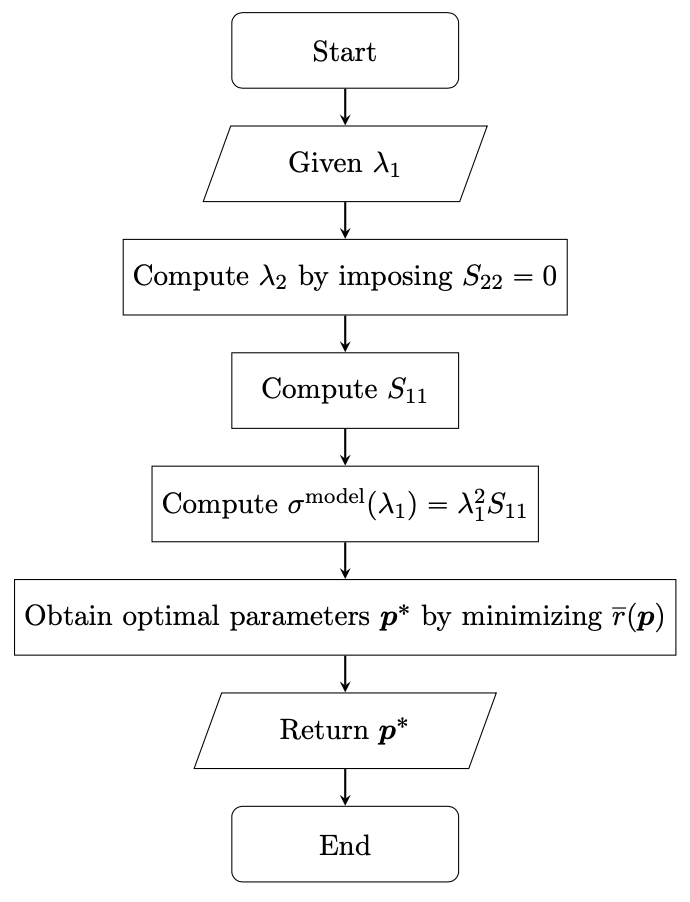
\includegraphics[width = 0.4\textwidth]{Flowchart.png}
    \end{center}
    \caption[Summary of the deterministic calibration.]{Summary of the procedure enabling the deterministic calibration of material parameters on the synthesized samples.}
    \label{fig:flowchart}
\end{figure}
Notice that the optimal values for the parameters involved in the stochastic formulation, gathered in a realization vector $\bfz^*$, are then obtained by using the changes of variables defined in Section \ref{Stochastic Model Homogeneous}.

The results of the adjusted material model and the digitally-generated data for the three layers are shown in Figs.~\ref{fig:det-fit-adv}, \ref{fig:det-fit-med}, and \ref{fig:det-fit-int}. 
\begin{figure}[ht!]
    \begin{center}
        \includegraphics[width = 0.48\textwidth]{Adv_Circ.pdf} \includegraphics[width = 0.48\textwidth]{Adv_Long.pdf}
    \end{center}
    \caption[Fitting results for the adventitia layer.]{Fitting results for the adventitia layer. The reference results are shown in solid black line, while the results obtained with the proposed model are shown in red solid line. Left panel: circumferential direction. Right panel: longitudinal direction.}
    \label{fig:det-fit-adv}
\end{figure}
\begin{figure}[ht!]
    \begin{center}
        \includegraphics[width = 0.48\textwidth]{Med_Circ.pdf} \includegraphics[width = 0.48\textwidth]{Med_Long.pdf}
    \end{center}
    \caption[Fitting results for the media layer.]{Fitting results for the media layer. The reference results are shown in solid black line, while the results obtained with the proposed model are shown in red solid line. Left panel: circumferential direction. Right panel: longitudinal direction.}
    \label{fig:det-fit-med}
\end{figure}
\begin{figure}[ht!]
    \begin{center}
        \includegraphics[width = 0.48\textwidth]{Int_Circ.pdf} \includegraphics[width = 0.48\textwidth]{Int_Long.pdf}
    \end{center}
    \caption[Fitting results for the intima layer.]{Fitting results for the intima layer. The reference results are shown in solid black line, while the results obtained with the proposed model are shown in red solid line. Left panel: circumferential direction. Right panel: longitudinal direction.}
    \label{fig:det-fit-int}
\end{figure}
It is seen that the model can reproduce the data very well, as expected given the similarities between the strain energy density functions used in this paper and in the reference work \cite{holzapfel2005determination} (which only differs in the isotropic contribution). The lists of material parameters thus obtained are provided for all layers in Table~\ref{tab:cal-par-det-adv}, \ref{tab:cal-par-det-med}, and \ref{tab:cal-par-det-int}. The mean averages for these parameters (in the order $\mu_1$, $\mu_2$, $\mu_4$, $\beta_4$, $\alpha$, and $\rho$) are provided for each layer below:
\begin{itemize}
    \item Adventitia: 6.5462 [kPa], 0.1034 [kPa], 21.3557 [kPa], 96.6721 [--], 1.1419 [rad], 0.5151 [--];
    \item Media: 1.2079 [kPa], 0.0230 [kPa], 10.7838 [kPa], 8.1899 [--], 0.3558 [rad], 0.2490 [--];
    \item Intima: 28.4956 [kPa], 0.4725 [kPa], 145.8811 [kPa], 177.3867 [--], 1.1096 [rad], 0.5044 [--].
\end{itemize}

\begin{table}[ht!]
\caption[Calibrated parameters for the adventitia layer.]{Calibrated parameters for the adventitia layer. Specimens numbers are associated with the results presented in \cite{holzapfel2005determination}. Note that the parameter $\mu_4$ here is half of the corresponding parameter in \cite{holzapfel2005determination}, given the expression for the strain energy density function.}
\label{tab:cal-par-det-adv}
\begin{center}
    \begin{tabular}{|c |c| c| c| c| c| c| c|} 
 \hline
 \quad Specimen \quad & \quad $\mu_1$ \quad & \quad $\mu_2$ \quad & \quad $\mu_4$ \quad & \quad $\beta_4$ \quad & \quad $\alpha$ \quad & \quad $\rho$ \quad & Error $\overline{r}(\bfp^*)$ \quad \\
 \quad \# \quad & [kPa] \quad & \quad [kPa] \quad & \quad [kPa] \quad & \quad [--] \quad & \quad [rad] \quad & \quad [--] \quad & $\times 10^{-6}$ \quad \\
 \cline{1-8} 
    1 & 3.8154 & 0.0952   & 16.2516  & 103.8667 & 1.2681 & 0.6503 & 0.3131\\
    2 & 2.2703 & 0.0471   & 6.9480  & 81.3985 & 1.1781 & 0.7510 & 0.8667\\
    3 & 4.8053 & 0.0395   & 33.6126 & 49.4776 & 1.0699 & 0.4999 & 0.1708\\
    5 & 9.1153 & 0.2103   & 41.0040 & 145.0781 & 0.9320 & 0.3998 & 0.8243\\
    6 & 7.7952 & 0.0571   & 12.6815 & 67.9862 & 1.2264 & 0.7003 & 0.1121\\
    8 & 2.0467 & 0.0833   & 18.8116 & 48.7029 & 1.1422 & 0.4040 & 0.2818 \\
    9 & 5.6493 & 0.2089   & 16.4234 & 167.2432 & 1.3151 & 0.2998 & 0.2761\\
    10 & 14.7392 & 0.0778 & 59.5418 & 214.0337 & 0.9320 & 0.6001 & 0.2067\\
    11 & 12.3502 & 0.1629 & 17.5735 & 84.9840 & 1.2083 & 0.6005 & 0.2450\\
    12 & 2.8631 & 0.1009  & 8.7606 & 68.4434 & 0.9597 & 0.4105 & 0.9009\\
    13 & 6.5583 & 0.0541  &  3.3039 & 32.1794 & 1.3297 & 0.3500 & 0.2420\\
 \hline 
\end{tabular}
\end{center}
\end{table}

\begin{table}[ht!]
\caption[Calibrated parameters for the media layer.]{Calibrated parameters for the media layer. Specimens numbers are associated with the results presented in \cite{holzapfel2005determination}. Note that the parameter $\mu_4$ here is half of the corresponding parameter in \cite{holzapfel2005determination}, given the expression for the strain energy density function.}
\label{tab:cal-par-det-med}
\begin{center}
    \begin{tabular}{|c |c| c| c| c| c| c| c|} 
 \hline
 \quad Specimen \quad & \quad $\mu_1$ \quad & \quad $\mu_2$ \quad & \quad $\mu_4$ \quad & \quad $\beta_4$ \quad & \quad $\alpha$ \quad & \quad $\rho$ \quad & Error $\overline{r}(\bfp^*)$ \quad \\
 \quad \# \quad & [kPa] \quad & \quad [kPa] \quad & \quad [kPa] \quad & \quad [--] \quad & \quad [rad] \quad & \quad [--] \quad & $\times 10^{-6}$ \quad \\
 \cline{1-8}
    1 & 0.9122 & 0.0094  & 6.6063  & 10.7580 & 0.3592 & 0.2476 & 0.2793\\
    2 & 1.0174 & 0.0269  & 12.8334  & 5.8988 & 0.4449 & 0.2970 & 0.2268\\
    3 & 1.7214 & 0.0236  & 10.4581  & 5.7353 & 0.3916 & 0.1967 & 0.2478\\
    4 & 1.5992 & 0.0109  &  13.1523 & 9.5337 & 0.4439 & 0.3980 & 0.1677\\
    5 & 2.4868 & 0.0223  & 8.3441  & 13.8411 & 0.2968 & 0.2000 & 0.2959\\
    6 & 0.6409 & 0.0338  & 15.2760  & 5.3399 & 0.3226 & 0.2987 & 0.2007\\
    7 & 0.8698 & 0.0246  & 12.4674  & 7.5124 & 0.2147 & 0.1500 & 0.2853\\
    8 & 0.2368 & 0.0313  &  13.9616 & 5.4142 & 0.1840 & 0.1993 & 0.1661\\
    9 & 2.2856 & 0.0119  &  4.2552  & 12.8970 & 0.4405 & 0.3032 & 0.1334\\
    10 & 0.7071 & 0.0531 & 15.5753 & 2.5561 & 0.2740 & 0.0986 & 0.1921\\
    11 & 1.1838 & 0.0117 & 6.5073 & 8.4201 & 0.5203 & 0.3015 & 0.3128\\
    12 & 0.8871 & 0.0263 & 10.7400 & 7.7343 & 0.3482 & 0.1480 & 0.2638\\
    13 & 1.1550 & 0.0130 & 10.0128 & 10.8277 & 0.3842 & 0.3984 & 0.2561\\
 \hline
\end{tabular}
\end{center}
\end{table}

\begin{table}[ht!]
\caption[Calibrated parameters for the intima layer.]{Calibrated parameters for the intima layer. Specimens numbers are associated with the results presented in \cite{holzapfel2005determination}. Note that the parameter $\mu_4$ here is half of the corresponding parameter in \cite{holzapfel2005determination}, given the expression for the strain energy density function.}
\label{tab:cal-par-det-int}
\begin{center}
    \begin{tabular}{|c |c| c| c| c| c| c| c|} 
 \hline
 \quad Specimen \quad & \quad $\mu_1$ \quad & \quad $\mu_2$ \quad & \quad $\mu_4$ \quad & \quad $\beta_4$ \quad & \quad $\alpha$ \quad & \quad $\rho$ \quad & Error $\overline{r}(\bfp^*)$ \quad \\
 \quad \# \quad & [kPa] \quad & \quad [kPa] \quad & \quad [kPa] \quad & \quad [--] \quad & \quad [rad] \quad & \quad [--] \quad & $\times 10^{-6}$ \quad \\
 \cline{1-8} 
   1 & 26.0930 &   1.0707 &  61.8350 & 180.6829  &  1.2129 &   0.5496 &  0.1064\\
   2 & 42.0952 &   0.1300 & 132.1545 & 286.9763  &  0.9372  &  0.6999 & 0.0253\\
   3 & 24.8050 &   0.2085 & 117.1730 & 176.7649  &  1.0085  &  0.5005 & 0.0233\\
   4 & 48.1296 &   2.2548 & 930.3108 & 454.7669  &  0.8168  &  0.3994 & 0.0235\\
   5 & 24.2734 &   0.1897 & 184.8636 & 342.9503  &  0.6965  &  0.7002 & 0.0266\\
   7 & 34.2402 &   0.1682  & 27.4200 &  92.7600  &  1.2620  &  0.3498 & 0.0307\\
   8 & 25.8023 &   0.1473  & 30.0657 & 110.3671  &  1.2950  &  0.3499 & 0.0253\\
   10 & 27.2055 &   0.1071 &  16.2175 &  72.3563  &  1.1521  &  0.3998 & 0.0223\\
   11 & 25.8057 &   0.1510 &  28.1253  & 77.8412  &  1.1570  &  0.4999 & 0.0256\\
   12 & 15.2380 &   0.5128 &  40.1371 &  73.7906  &  1.3643  &  0.6499 & 0.0203\\
   13 & 19.7643 &   0.2577 &   36.3891 &  81.9973 &   1.3036  &  0.4498 & 0.0263\\
 \hline 
\end{tabular}
\end{center}
\end{table}


\subsection{Calibration of the Stochastic Model} \label{subsec:sto-calibration}

Since the components of $\bfZ$ are statistically independent, we use the maximum likelihood method to calibrate the hyperparameters for each random variable. Denote by $\boldsymbol{s}$ the vector gathering the set of hyperparameters for a given component of $\bfZ$ in the stochastic model. The optimal value of $\boldsymbol{s}$ is then obtained as
\begin{align}
    \hat{\boldsymbol{s}} &= \text{argmax}_{\boldsymbol{s} \in \mathcal{C}_{\boldsymbol{s}}} \quad \mathcal{L}(\boldsymbol{s}; \bfy)\,,
\end{align}
where $\mathcal{C}_{\boldsymbol{s}}$ denotes the parameter space, $\mathcal{L}$ is the likelihood function, and $\bfy$ is the observed data sample. The values of all hyperparameters are given in Table~\ref{tab:hyperparameters}, and the associated probability density functions (together with samples) are shown in Figs.~\ref{fig:MLE-Set-1}, \ref{fig:MLE-Set-2}, and \ref{fig:MLE-Set-3}.
\begin{table}[ht!]
\caption[Hyperparameters estimated with the maximum likelihood method.]{Hyperparameters estimated with the maximum likelihood method for all layers.}
\label{tab:hyperparameters}
\begin{center}
    \begin{tabular}{|c|c|c|c|} 
 \hline
 \quad Parameter \quad & \quad $\hat{\boldsymbol{s}}$ (adventitia) \quad & \quad $\hat{\boldsymbol{s}}$ (media) \quad & \quad $\hat{\boldsymbol{s}}$ (intima) \quad \\
 \cline{1-4} 
    $C_2$ & $(2.9459, 4.6266)$  & $(3.6841, 0.7075)$   & $(1.4120, 35.8575)$\\
    $V$   & $(1.6574, 99.5985)$ & $(5.9044, 22.4244)$  & $(0.6364, 1.645 \times 10^3)$\\
    $B_4$ & $(3.5262, 27.4153)$ & $(5.2736, 1.5154)$   & $(1.1744, 129.0230)$\\
    $U$   & $(48.4729, 2.5140)$ & $(14.4793, 1.1649)$  & $(34.4290, 1.43553)$\\
    $R$   & $(5.8703, 5.5101)$  & $(6.25578, 19.3627)$ & $(3.1868, 1.9178)$\\
    $T$   & $(17.7955, 6.6881)$ & $(8.8830, 30.5876)$  & $(4.5830, 5.2297)$\\
 \hline 
\end{tabular}
\end{center}
\end{table}
In practice, these hyperparameters can used to generate mathematically-consistent virtual samples. 

\begin{figure}[ht!]
    \begin{center}
        \includegraphics[width = 0.48\textwidth]{MLE-C2.pdf} \includegraphics[width = 0.48\textwidth]{MLE-V.pdf}
    \end{center}
    \caption[Probability density functions (PDFs) of $C_2$ and $V$.]{Probability density functions (PDFs), with hyperparameters estimated with the maximum likelihood method, and experimental samples. Left panel: random variable $C_2$. Right panel: random variable $V$.}
    \label{fig:MLE-Set-1}
\end{figure}
\begin{figure}[ht!]
    \begin{center}
        \includegraphics[width = 0.48\textwidth]{MLE-B4.pdf} \includegraphics[width = 0.48\textwidth]{MLE-U.pdf}
    \end{center}
    \caption[Probability density functions (PDFs) of $B_2$ and $U$.]{Probability density functions (PDFs), with hyperparameters estimated with the maximum likelihood method, and experimental samples. Left panel: random variable $B_2$. Right panel: random variable $U$.}
    \label{fig:MLE-Set-2}
\end{figure}
\begin{figure}[ht!]
    \begin{center}
        \includegraphics[width = 0.48\textwidth]{MLE-T.pdf} \includegraphics[width = 0.48\textwidth]{MLE-R.pdf}
    \end{center}
    \caption[Probability density functions (PDFs) of $T$ and $R$.]{Probability density functions (PDFs), with hyperparameters estimated with the maximum likelihood method, and experimental samples. Left panel: random variable $T$. Right panel: random variable $R$.}
    \label{fig:MLE-Set-3}
\end{figure}

Using these results, new samples of $\bfZ$ can be generated and pulled back to obtain samples of the primary parameters defining the strain energy density function. Using $10^{6}$ samples, the following mean values were obtained for these parameters:
\begin{itemize}
    \item Adventitia: 6.4760 [kPa], 0.1297 [kPa], 24.0164 [kPa], 96.4960 [--], 1.1426 [rad], 0.5172 [--];
    \item Media: 1.2076 [kPa], 0.0379 [kPa], 11.1438 [kPa], 8.0084 [--], 0.3539 [rad], 0.2440 [--];
    \item Intima: 24.2965 [kPa], 0.3893 [kPa], 136.2482 [kPa], 151.3538 [--], 0.9806 [rad], 0.4672 [--].
\end{itemize}
It is seen that these results slightly differ from the ones reported in Section \ref{subsec:det-calibration}, where mean averaging was used instead of a maximum likelihood estimator. In order to qualitatively assess this result, the mean responses obtained by using either parameterization (that is, the one provided in Section \ref{subsec:det-calibration} or the one given above) are shown for all layers and both directions in Figs.~\ref{fig:mean-adv}, \ref{fig:mean-med}, and \ref{fig:mean-int}. The difference between the two responses is most noticeable for the intima layer, due to the strong stiffening effect. Finally, 95\% confidence intervals were estimated with the model, using 100,000 independent samples. These intervals are also displayed in Figs.~\ref{fig:mean-adv}, \ref{fig:mean-med}, and \ref{fig:mean-int}, and are seen to capture experimental variability with reasonable accuracy.
\begin{figure}[ht!]
    \begin{center}
        \includegraphics[width = 0.48\textwidth]{MeanCI-Adv-Circ.pdf} \includegraphics[width = 0.48\textwidth]{MeanCI-Adv-Long.pdf}
    \end{center}
    \caption[Experimental results obtained for the adventitia layer.]{Experimental results (black solid lines), mean responses obtained for the adventitia layer by using either the MLE-based estimate (blue solid line) or a mean average (blue dashed line), and 95\% confidence interval (red solid line). Left panel: circumferential direction. Right panel: longitudinal direction.}
    \label{fig:mean-adv}
\end{figure}
\begin{figure}[ht!]
    \begin{center}
        \includegraphics[width = 0.48\textwidth]{MeanCI-Med-Circ.pdf} \includegraphics[width = 0.48\textwidth]{MeanCI-Med-Long.pdf}
    \end{center}
    \caption[Experimental results obtained for the media layer.]{Experimental results (black solid lines), mean responses obtained for the media layer by using either the MLE-based estimate (blue solid line) or a mean average (blue dashed line), and 95\% confidence interval (red solid line). Left panel: circumferential direction. Right panel: longitudinal direction.}
    \label{fig:mean-med}
\end{figure}
\begin{figure}[ht!]
    \begin{center}
        \includegraphics[width = 0.48\textwidth]{MeanCI-Int-Circ.pdf} \includegraphics[width = 0.48\textwidth]{MeanCI-Int-Long.pdf}
    \end{center}
    \caption[Experimental results obtained for the intima layer.]{Experimental results (black solid lines), mean responses obtained for the intima layer by using either the MLE-based estimate (blue solid line) or a mean average (blue dashed line), and 95\% confidence interval (red solid line). Left panel: circumferential direction. Right panel: longitudinal direction.}
    \label{fig:mean-int}
\end{figure}

\section{Uncertainty Propagation} \label{sec:uncertainty-propagation}


\subsection{Definition of the Random Field Model on a Patient-Specific Geometry}

In this section, we consider the propagation of the uncertainties associated with the proposed random field model on a patient-specific geometry. Without loss of generality, we assume that the latter corresponds to the adventitia layer (which is the outermost layer in the arterial wall). We use the domain studied in \cite{STABER201894}, which was obtained by postprocessing the inner surface available as file 0098 in the Aneurisk database \cite{AneuriskWeb}. The domain is about $12$ [mm] long and is shown in Fig.~\ref{fig:geometry}. Details about discretization are provided in Section \ref{subsec:SFEM-propagation}.
\begin{figure}[ht!]
    \begin{center}
        \includegraphics[trim = {5cm 7cm 5cm 7cm}, clip, width = 0.48\textwidth]{Artery3D.pdf} \includegraphics[trim = {5cm 5cm 5cm 7cm}, clip, width = 0.4\textwidth]{ArterySlice.pdf}
    \end{center}
    \caption[Three-dimensional and slice views of the arterial wall.]{Three-dimensional and slice views of the arterial wall, computed from \cite{AneuriskWeb}.}
    \label{fig:geometry}
\end{figure}

In order to define the latent Gaussian field $\{{\bf \Xi}(\bfx), \bfx \in B\}$, we use the SPDE approach introduced in Section \ref{subsec:def-Gaussian} (with $\alpha = 2$). As a preliminary step, we use the Laplace-Dirichlet Rule-Based algorithm \cite{Bayer2012,Augustin2014} to define some local orientation fields involved in the parameterization of the diffusion $[H]$. Specifically, we introduce the vector fields $\bfx \mapsto \bfe^{(1)}(\bfx)$ and $\bfx \mapsto \bfe^{(2)}(\bfx)$ defined as
\begin{equation}
\bs{e}^{(1)}(\bs{x}) = \frac{\nabla\Psi_2(\bs{x})}{ \| \nabla \Psi_2(\bs{x}) \| }~, \quad \bs{e}^{(2)}(\bs{x}) = \bs{e}^{(3)}(\bs{x}) \times \bs{e}^{(1)}(\bs{x})~, \quad \bs{e}^{(3)}(\bs{x}) = \frac{\nabla \Psi_1(\bs{x})}{ \| \nabla \Psi_1(\bs{x}) \| }~,
\end{equation}
where $\bs{x} \mapsto \Psi_1(\bs{x})$ satisfies 
\begin{equation}
\Delta \Psi_1({\bs{x}}) = 0~, \quad \forall \, {\bs{x}} \in B~,
\end{equation}
with $\Psi_1({\bs{x}}) = 0$ on the inlet surface and $\Psi_1({\bs{x}}) = 1$ on the outlet surface, and $\bs{x} \mapsto \Psi_2(\bs{x})$ is the solution to a similar Laplace problem with $\Psi_2({\bs{x}}) = 0$ on the inner surface and $\Psi_2({\bs{x}}) = 1$ on the outer surface \cite{STABER201894}.

As a first step, we then consider the Gaussian component associated with the angle random field $\{A(\bfx), \bfx \in B\}$ and use a SPDE where the diffusion field is defined as
\begin{equation}\label{eq:def-H-final-application}
    \bs{D}(\bfx) = \kappa \bs{I} + \tau_1 \hat{\bfe}^{(1)}(\bfx) \otimes \hat{\bfe}^{(1)}(\bfx) + \tau_2 \hat{\bfe}^{(2)}(\bfx) \otimes \hat{\bfe}^{(2)}(\bfx)\,,
\end{equation}
where
\begin{equation}    
    \hat{\bfe}^{(1)}(\bfx) = \cos(\underline{a}) \bfe^{(1)}(\bfx) + \sin(\underline{a})\bfe^{(2)}(\bfx)\,, \quad \hat{\bfe}^{(2)}(\bfx) = \cos(\underline{a}) \bfe^{(1)}(\bfx) - \sin(\underline{a})\bfe^{(2)}(\bfx)\,,
\end{equation}
and $\underline{a}$ is the mean value for the angle obtained from the calibrated step detailed in Section \ref{sec:calibration} (for the adventitia layer). In effect, this introduces some waviness effect in the local orientation, for both the anisotropic mechanical behavior and covariance structure, which can be related to waviness in the orientation of collagen fibers at a finer scale. By construction, this modeling feature can be turned off by setting the associated coefficient of variation to zero.

Next, and for a \textit{given} sample $\bfx \mapsto a(\bfx, \theta)$ of the angle random field thus obtained, with $\theta \in \Theta$, the latent Gaussian components associated with the other material random fields are defined and sampled by solving the SPDE with the diffusion taken as in Eq.~\eqref{eq:def-H-final-application}, where the orientation vectors are now defined as
\begin{equation}    
    \hat{\bfe}^{(1)}(\bfx) = \cos(a(\bfx, \theta)) \bfe^{(1)}(\bfx) + \sin(a(\bfx, \theta))\bfe^{(2)}(\bfx)
\end{equation}
and
\begin{equation}    
 \hat{\bfe}^{(2)}(\bfx) = \cos(a(\bfx, \theta)) \bfe^{(1)}(\bfx) - \sin(a(\bfx, \theta))\bfe^{(2)}(\bfx)\,.
\end{equation}

Following the methodology of construction presented in Section \ref{sec:sto-heterogeneous}, we now proceed with the specification of the hyperparameters defining the transport map $H$. A natural choice here is to use the parameters identified in Section \ref{subsec:sto-calibration}; see Table~\ref{tab:hyperparameters}. However, the associated probability density functions represent inter-patient variability and would therefore generate unrealistically large (intra-patient) spatial fluctuations. For this reason, we propose to preserve the mean values estimated at the calibration stage, and to scale the coefficients of variation in a proportional manner (meaning that properties that exhibit larger fluctuations still present larger spatial variations). The proposed values for these coefficients of variation are listed in Table~\ref{tab:scaled-hyperparameters}.
\begin{table}[ht!]
\caption[Scaled coefficients of variation of the random variables.]{Scaled values for the coefficients of variation of the random variables.}
\label{tab:scaled-hyperparameters}
\begin{center}
    \begin{tabular}{|c|c|c|} 
 \hline
 \quad Parameter \quad & \quad Data-based coefficient of variation \quad & \quad Scaled coefficient of variation \quad \\
 \cline{1-3} 
    $C_2$ & $0.5826$  & $0.15$ \\
    $V$   & $0.7768$ & $0.2$ \\
    $B_4$ & $0.5325$ & $0.1371$ \\
    $U$   & $0.0316$ & $0.0081$ \\
    $R$   & $0.2753$  & $0.0709$ \\
    $T$   & $0.1214$ & $0.0313$ \\
 \hline 
 \end{tabular}
\end{center}
\end{table}
The corresponding set of hyperparameters are provided in Table~\ref{tab:hyperparameters-scaled}.
\begin{table}[ht!]
\caption[Hyperparameters corresponding to the scaled coefficients of variation.]{Hyperparameters corresponding to the scaled coefficients of variation (given in the far-right column in Table~\ref{tab:scaled-hyperparameters}).}
\label{tab:hyperparameters-scaled}
\begin{center}
    \begin{tabular}{|c|c|} 
 \hline
 \quad Parameter \quad & \quad $\hat{\boldsymbol{s}}$ (adventitia) \quad \\
 \cline{1-2} 
    $C_2$ & $(44.4351, 0.3067)$\\
    $V$   & $(25, 6.6031)$\\
    $B_4$ & $(53.1877, 1.8176)$\\
    $U$   & $(744.5323, 38.6146)$\\
    $R$   & $(95.81, 89.9306)$\\
    $T$   & $(278.6547, 104.727)$\\
 \hline 
\end{tabular}
\end{center}
\end{table}

Realizations of the random fields of material parameters are shown in Figs.~\ref{fig:samples-1}, \ref{fig:samples-2}, and \ref{fig:samples-3}, for $\gamma = 1$, $\kappa = 0.1$, and $\tau_1 = \tau_2 = 10$. These values are selected for the sake of illustration to induce moderate correlation ranges on the arterial wall. The identification of such parameters requires spatial data that are not currently available for the proposed application (and may be obtained using, e.g., ultrasound characterization techniques) and is left for future work.
\begin{figure}[ht!]
    \begin{center}
        
    \includegraphics[trim = {6cm 3cm 6cm 5cm}, clip, width = 0.48\textwidth]{Sample_G1.pdf} \includegraphics[trim = {6cm 3cm 6cm 5cm}, clip, width = 0.48\textwidth]{Sample_G2.pdf}
    \end{center}
    \caption[Sample of $\{G_1(\bfx), \bfx \in B\}$ and $\{G_2(\bfx), \bfx \in B\}$ in the adventitia layer.]{Sample of $\{G_1(\bfx), \bfx \in B\}$ (left) and $\{G_2(\bfx), \bfx \in B\}$ (right) in the adventitia layer.}
    \label{fig:samples-1}
\end{figure}

\begin{figure}[ht!]
    \begin{center}
        \includegraphics[trim = {6cm 3cm 6cm 5cm}, clip, width = 0.48\textwidth]{Sample_G4.pdf} \includegraphics[trim = {6cm 3cm 6cm 5cm}, clip, width = 0.48\textwidth]{Sample_B4.pdf}
    \end{center}
    \caption[Sample of $\{G_4(\bfx), \bfx \in B\}$ and $\{B_4(\bfx), \bfx \in B\}$ in the adventitia layer.]{Sample of $\{G_4(\bfx), \bfx \in B\}$ (left) and $\{B_4(\bfx), \bfx \in B\}$ (right) in the adventitia layer.}
    \label{fig:samples-2}
\end{figure}

\begin{figure}[ht!]
    \begin{center}
        \includegraphics[trim = {6cm 3cm 6cm 5cm}, clip, width = 0.48\textwidth]{Sample_R.pdf} \includegraphics[trim = {6cm 3cm 6cm 5cm}, clip, width = 0.48\textwidth]{Sample_A.pdf}
    \end{center}
    \caption[Sample of $\{R(\bfx), \bfx \in B\}$ and $\{A(\bfx), \bfx \in B\}$ in the adventitia layer.]{Sample of $\{R(\bfx), \bfx \in B\}$ (left) and $\{A(\bfx), \bfx \in B\}$ (right) in the adventitia layer.}
    \label{fig:samples-3}
\end{figure}

\subsection{Propagation of Uncertainties}\label{subsec:SFEM-propagation}

In this work, the nonlinear boundary value problem is solved by the finite element method, using a total Lagrangian formulation and a three-field formulation ($\mathbb{P}_2$-$\mathbb{P}_0$-$\mathbb{P}_0$ discretization) to handle quasi-incompressibility \cite{wriggers2008nonlinear}. The geometry shown in Fig.~\ref{fig:geometry} is discretized with a mesh containing $297,828$ cells and $432,250$ nodes. An inflating pressure of 1 [kPa] is applied on the inner layer and sliding displacement boundary conditions are prescribed on the inlet and outlet surfaces (the system is made statically determined by restricting additional degrees of freedom at two nodes located on the outlet surface). Implementation was performed within the MOOSE finite element framework \cite{permann2020moose} and code verification was conducted through the method of manufactured solution (described in \ref{app:VV-artery}).  

Given the random field modeling setting, a Monte-Carlo approach was used to propagate uncertainties (see the remark at the end of this section). Interested readers are referred to \cite{Ghanem2017} for a comprehensive review on alternative stochastic solvers (see \cite{hauseux2018quantifying} for a specific discussion regarding hyperelastic materials). Parallel computing with 36 cores was used to accelerate the deterministic runs.

The fields of mean values and coefficients of variation are shown in Fig.~\ref{fig:vonMises}.
\begin{figure}[ht!]
    \begin{center}
        \includegraphics[trim = {6cm 3cm 6cm 5cm}, clip, width = 0.48\textwidth]{Mean-vMStress.pdf} \includegraphics[trim = {6cm 3cm 6cm 5cm}, clip, width = 0.48\textwidth]{CV-vMStress.pdf}
    \end{center}
    \caption[Mean and coefficient of variation for the von Mises stress.]{Mean (left) and coefficient of variation (right) for the von Mises stress (slice views).}
    \label{fig:vonMises}
\end{figure}
Substantial spatial variations are observed in both fields and localization is less pronounced than in the results presented in \cite{STABER201894}---as angular waviness tends to mitigate that effect. Values for the mean field range from 0.15 to 40 [kPa], while values for the coefficient of variation are distributed between 0.025 to 0.42. While these quantitative results are conditioned by the proposed scaling in variance (defined in Tab.~\ref{tab:scaled-hyperparameters}) and the selected values for the hyperparameters defining the latent Gaussian fields, they show the impact of material variability on the response of the arterial wall. Additional work assimilating spatial data is therefore necessary to refine the propagation analysis and translate the results into practical applications: the proposed modeling framework is a first step towards that goal.

\begin{remark}
The usual spectral approach to uncertainty propagation consists in representing the random fields through Karhunen-Lo\`eve expansions and in seeking a polynomial chaos surrogate in terms of the reduced variables. It is therefore instructive to analyze a posteriori the dimension obtained for a given field defined and sampled through the SPDE approach, say $\{G_1(\bfx), \bfx \in B\}$. The graph of the standard error function $n \mapsto \textnormal{Conv}(n)$, where
\begin{equation}
    \textnormal{Conv}(n) = 1 - \frac{\sum_{i = 1}^{n} \lambda_i}{\textnormal{tr}(\textnormal{Cov}\{G_1\})}
\end{equation}
and the covariance matrix $\textnormal{Cov}\{G_1\}$ (and its eigenvalues $\{\lambda_i\}_{i \geq 1}$) are computed by using a singular value decomposition on the matrix of centered samples (200 samples are used here), is shown in Fig.~\ref{fig:conv}.
\begin{figure}[ht!]
    \begin{center}
        \includegraphics[width = 0.5\textwidth]{ConvN.pdf}
    \end{center}
    \caption[Graph of the function $n \mapsto \textnormal{Conv}(n)$.]{Graph of the function $n \mapsto \textnormal{Conv}(n)$.}
    \label{fig:conv}
\end{figure}
Retaining a truncation threshold of $0.01$ leads to a reduced dimension of 158, which suggests---given that six random fields are involved in the parameterization of the stochastic strain energy density function---a very high-dimensional setting for propagation through collocation-type approaches.
\end{remark}